\newpage
\section{Basic Functionality}

\subsection{VNC Access} \label{sec:vnc}

We use the graphical desktop-sharing system \href{https://en.wikipedia.org/wiki/Virtual_Network_Computing}{VNC} to manage access to the tabletop systems. VNC should be used for both in-person and remote work.

\begin{enumerate}
    \item   Install a free VNC application such as \href{https://tigervnc.org/}{tigervnc}.
    \item   Ensure you are connected to the Stanford network (use VPN if off-campus).
    \item   \label{step:login} Use VNC to connect to one of the tabletop systems using the login information below. Figure \ref{fig:vnc} shows an example.
    \begin{itemize}
        \item   User: Ocra1, VNC: mrtabletop:1, Pitaya IP: 192.168.1.84, password: Initpw123
        \item   User: Ocra2, VNC: mrtabletop:2, Pitaya IP: 192.168.1.83, password: Initpw123
        \item   User: Ocra3, VNC: mrtabletop:3, Pitaya IP: 192.168.1.82, password: Initpw123
    \end{itemize}
\end{enumerate}

\begin{wrapfigure}{r}{0.4\textwidth}
    \centering
    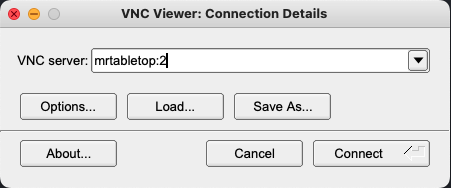
\includegraphics[width=0.36\textwidth]{vnc-example}
    \captionsetup{width=.36\textwidth}
    \caption{\label{fig:vnc}Example of a VNC connection interface.}
\end{wrapfigure}

Troubleshooting tips:
\begin{itemize}
    \item   Make sure you are the only person logged into the machine that you are trying to use. The machines won’t respond well if multiple users are using them and running sequences simultaneously.
    \item   If at any point the Pitaya stops responding or the sequences don’t run properly, you can restart the Pitaya remotely via the following steps:
    \begin{enumerate}
        \item   From the mrtabletop machine, ssh in to the appropriate Pitaya with the command \texttt{ssh root@192.168.1.xx}. (replace xx with IP suffix from step \ref{step:login}). There shouldn’t be a password prompt.
        \item   Once you are logged in, run the command \texttt{reboot}. The Pitaya will automatically restart and your ssh session will be terminated.
        \item   After the Pitaya reboots try running a simple test sequence. An easy sequence to run as a debugging step is a spin-echo.
    \end{enumerate}
\end{itemize}

% \subsection{System Start-up}

% \emph{Under normal circumstances the tabletop system will be powered on already and you can skip ahead to section \ref{sec:relax-program}.}

% Before beginning the startup procedure, ensure all boxes in the OCRA stack are OFF and the Raspberry Pi is unplugged.

% \begin{enumerate}
%     \item Switch the console box \textbf{on}.
%     \item Switch the gradient amplifier \textbf{on}. Press and hold the \textbf{Reset} button until the indicator lights turn green.
%     \item Plug in the Raspberry Pi. Login with password \texttt{raspberry}.
%     %\item Navigate to \texttt{/home/pi/Relax2} and double-click on \texttt{Relax2\_main.py} to open. Click the green arrow in the code editor to run the program.
%     %\item A dialog box will appear prompting you to select an IP address. Use the default IP address and click \textbf{Connect}.
%     %\item Observe the Relax 2.0 main menu (Figure \ref{fig:gui-menu}).
% \end{enumerate}

\begin{wrapfigure}{r}{0.4\textwidth}%this figure will be at the right
    \centering
    %\vspace{-15mm}
    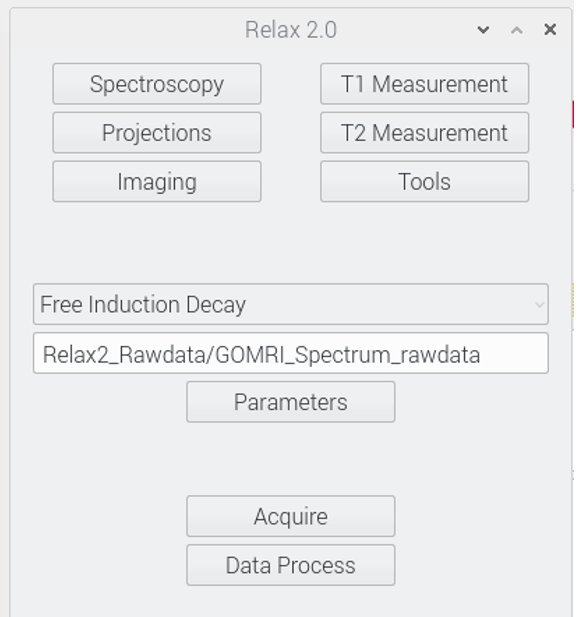
\includegraphics[width=0.36\textwidth]{gui-menu}
    \captionsetup{width=.36\textwidth}
    \caption{\label{fig:gui-menu}Relax 2.0 main menu.}
    %\vspace{-10mm}
\end{wrapfigure}

\subsection{Relax 2.0 Program} \label{sec:relax-program}

To run the Relax 2.0 program:

\begin{enumerate}
    \item   Open a terminal window.
    \item   Navigate to the program directory:
    
    \texttt{cd /home/ocra\#/Documents/221120\_Relax2}
    
    (\emph{replace \# appropriately})

    \item   Run the program:
    
    \texttt{python Relax2\_main.py}.

    \item   Enter the appropriate IP address (refer to section \ref{sec:vnc}).
    
\end{enumerate}

The Relax 2.0 main menu (Figure \ref{fig:gui-menu}) is the starting point for all experiments in this lab. The top 6 buttons toggle between broad categories of scans such as spectroscopy and projection imaging. The drop-down menu lists specific pulse sequences within the selected scan category. A typical workflow involves picking a category and a sequence, then modifying the sequence parameters over a series of acquisitions. These latter operations are explained below.

\textbf{Parameters} opens a window listing all mutable sequence parameters (e.g. echo time TE, repetition time TR) \emph{for all possible sequences}. Note that many of these parameters many not actually be used for a given sequence. This is an idiosyncrasy of the program that can be confusing. The lab manual should always tell you exactly which parameters to modify, but if there is any ambiguity don't hesitate to ask.

\textbf{Acquire} runs the selected sequence with the current parameter set. Unlike most scanners, expect this to run \emph{silently}.

\textbf{Data Process} operates on the raw data captured by the most recent \textbf{Acquire} event, calling any reconstruction and post processing routines associated with the selected sequence.

\subsection{Data Export}
\noindent{}In this lab you will capture experimental outputs in the form of screenshots and/or text files.

With a VNC connection you can capture screenshots of the remote desktop view with your own computer. This will be the primary mechanism for documenting your progress through the lab (e.g. saving plots and images), so make sure you have this working smoothly before you begin.

% \emph{Without a VNC connection}, if you access the Raspberry Pi directly then screenshots can be captured by opening a terminal window and using the \texttt{scrot} command. For example, \texttt{scrot filename.png} will save a screenshot to \texttt{filename.png} in the current working directory. Append a path to \texttt{filename.png} if you would like to specify some other directory.

Raw data and image data (if saved) are written to text files in the folders \texttt{Relax2\_Rawdata} and \texttt{Relax2\_Imagedata} folders respectively, both located in the same directory as \texttt{Relax2\_main.py}. You can change the folder or filename to prevent overwrite by editing the path in the field below the drop-down menu.

Finally, you can use a USB drive to transfer any files on the Raspberry Pi to another computer. To this end there will be one USB drive available for use \emph{in lab}. Please take care to erase the drive and leave it next to the phantom tray at the end of each session.
